I still need to spend a lot of time with OSM, networkx, and the London data store. 
OSM has street network data, bike network data and some road characteristics. 
Networkx should be able to turn this data into a usable file. 
The London data store has traffic incident data but I haven't found data with exact locations yet
There is traffic volume data but it's at a few thousand observation points, so a continuous data set needs to be estimated. 
I think OSM is my only source for street characteristics, not clear that it's accurate or up to date.
Official data for cycle infrastructure is from 2014: \href{https://data.gov.uk/dataset/47f0a282-3356-4530-8e7b-f67aaf4bec63/cycle-routes}{link}
This says it's updated and maybe integrated into OSM? \href{https://www.cyclestreets.net/blog/category/open-data/}{link}
Press release about data set \href{https://www.london.gov.uk/press-releases/mayoral/action-plan-to-get-more-londoners-cycling}{link}
But no actual data. Seems like OSM is the delivery mechanism, unclear how integrated the data is into OSM. 


\subsection{Open Street Map}


Open street map provides community generated geospatial data. This data is accessible via the overpass API from several hosts. 
Geoff Boeing describes using th OSM API query language as "notoriously difficult". \cite{osmnx}

https://www.nomisweb.co.uk/datasets/ks015

Accessing Open Street Map via the Overpass API is ``notoriously difficult'' Cite G Boeing. 

Open Street Map is a mapping project started in 2004 to collect volunteered geographic information. It consists of geometries drawn by users, either in person, as they travel through a city or remotely, looking at donated satelite images of cities. 

Cite OSM wiki page
https://en.wikipedia.org/wiki/OpenStreetMap

Second to the actual geometry of a "way", streets and paths, node, single point on the map, or relation, collection of ways nodes and other relations are tags. Tags specify what a particular geometry is, what its characteristics are, and rules for use or other characteristics of the geometry. This allows for differentiation on the map between public and private areas, specification of what exactly a node is referencing, an intersection, mailbox, or a business location, or the type of traffic allowed or commonly seen on a street way. 

There are four possible problems with Open Street Map, missing geometries, inaccurate geometries, missing tags and inaccurate tags. The review of literature will provide detail on attempts to measure the accuracy of the data in Open Street Map. 



Using data from Open street map is difficult. 

Compare Relation = cycleway to a list of edges and nodes tagged cycleway

Adding living streets and residential streets don't do much. 

Part of the problem is the lack of consistent tagging, it only takes one line segment missing a tag to disconnect two nodes,

but this also reflects the fact that getting somewhere within London nearly always requires leaving cycle infrastructure at some point and using main roads. 

The importance of this consideration will be shown using a percolation style analysis of the network, adding busier and busier roads to the network and considering the largest connected component. 


%%%%%%%%
% image of OSM London cycle network by relation
% image of OSM London cycle network by tag
% image of OSM missing tag situation from Overpass turbo
% image of same location street view
% image of OSM implied cycle infrastructure
% image of real street without cycle infrastructure. 
%%%%%%%%%%%%%

Two basic problems for using OSM data to define cycling networks were found. The first is that defining the network by relation exagerates the network, the second is that relying on the metadata tags of individual features understates the cycle network. Looking at OSM it is clear that the relations identifying bike routes are not reflecting sets of ways and nodes with a given tag, or reflecting streets and intersections where cycling is meaningfully safer than other streets and intersection. At the same time, it is clear that there are many ways and nodes that are more accomodating to cyclists than their OSM metadata indicates. 

In the case of the relation, Quietway XXX was examined in person. figure XXX shows an image of Brandon rd, a part of the quiet way. this way is tagged
Brandon rd is part of OSM relation XXX the Hackney Camden cycle route.  this road though, as can been seen in the image, has no actual cycle inrastructure. This in Open street map, it is tagged as an unclassified highway. There is a tag noting the max speed is 20 mph. Data collected for 20 mph streets found that as many as 80\% of drivers exceeded these limits. 
https://www.thesun.co.uk/news/7253694/20-mph-zones-cause-more-deaths/

In other cases, osm underestimates the quality of cycling infrastructure. for instance the intersection of Mile end Road and Cambridge Health Road in the borough of tower hamlets is a high traffic intersection both for automobiles and for cyclists. It is an integral part of the Stratford to Aldgate cycle super highway. This intersection has been reworked to be safer for cyclists. In open street map though, it i labeled a "trunk" highway, due to its high traffic nature. It is way 7058092014. There is also a tag cycleway:left=lane indicating that there is a cyclelane on the left side of the street. 

\cite{osm}

\subsection{A Close Look at an Open Street Map Case Study}

\begin{figure}
\centering
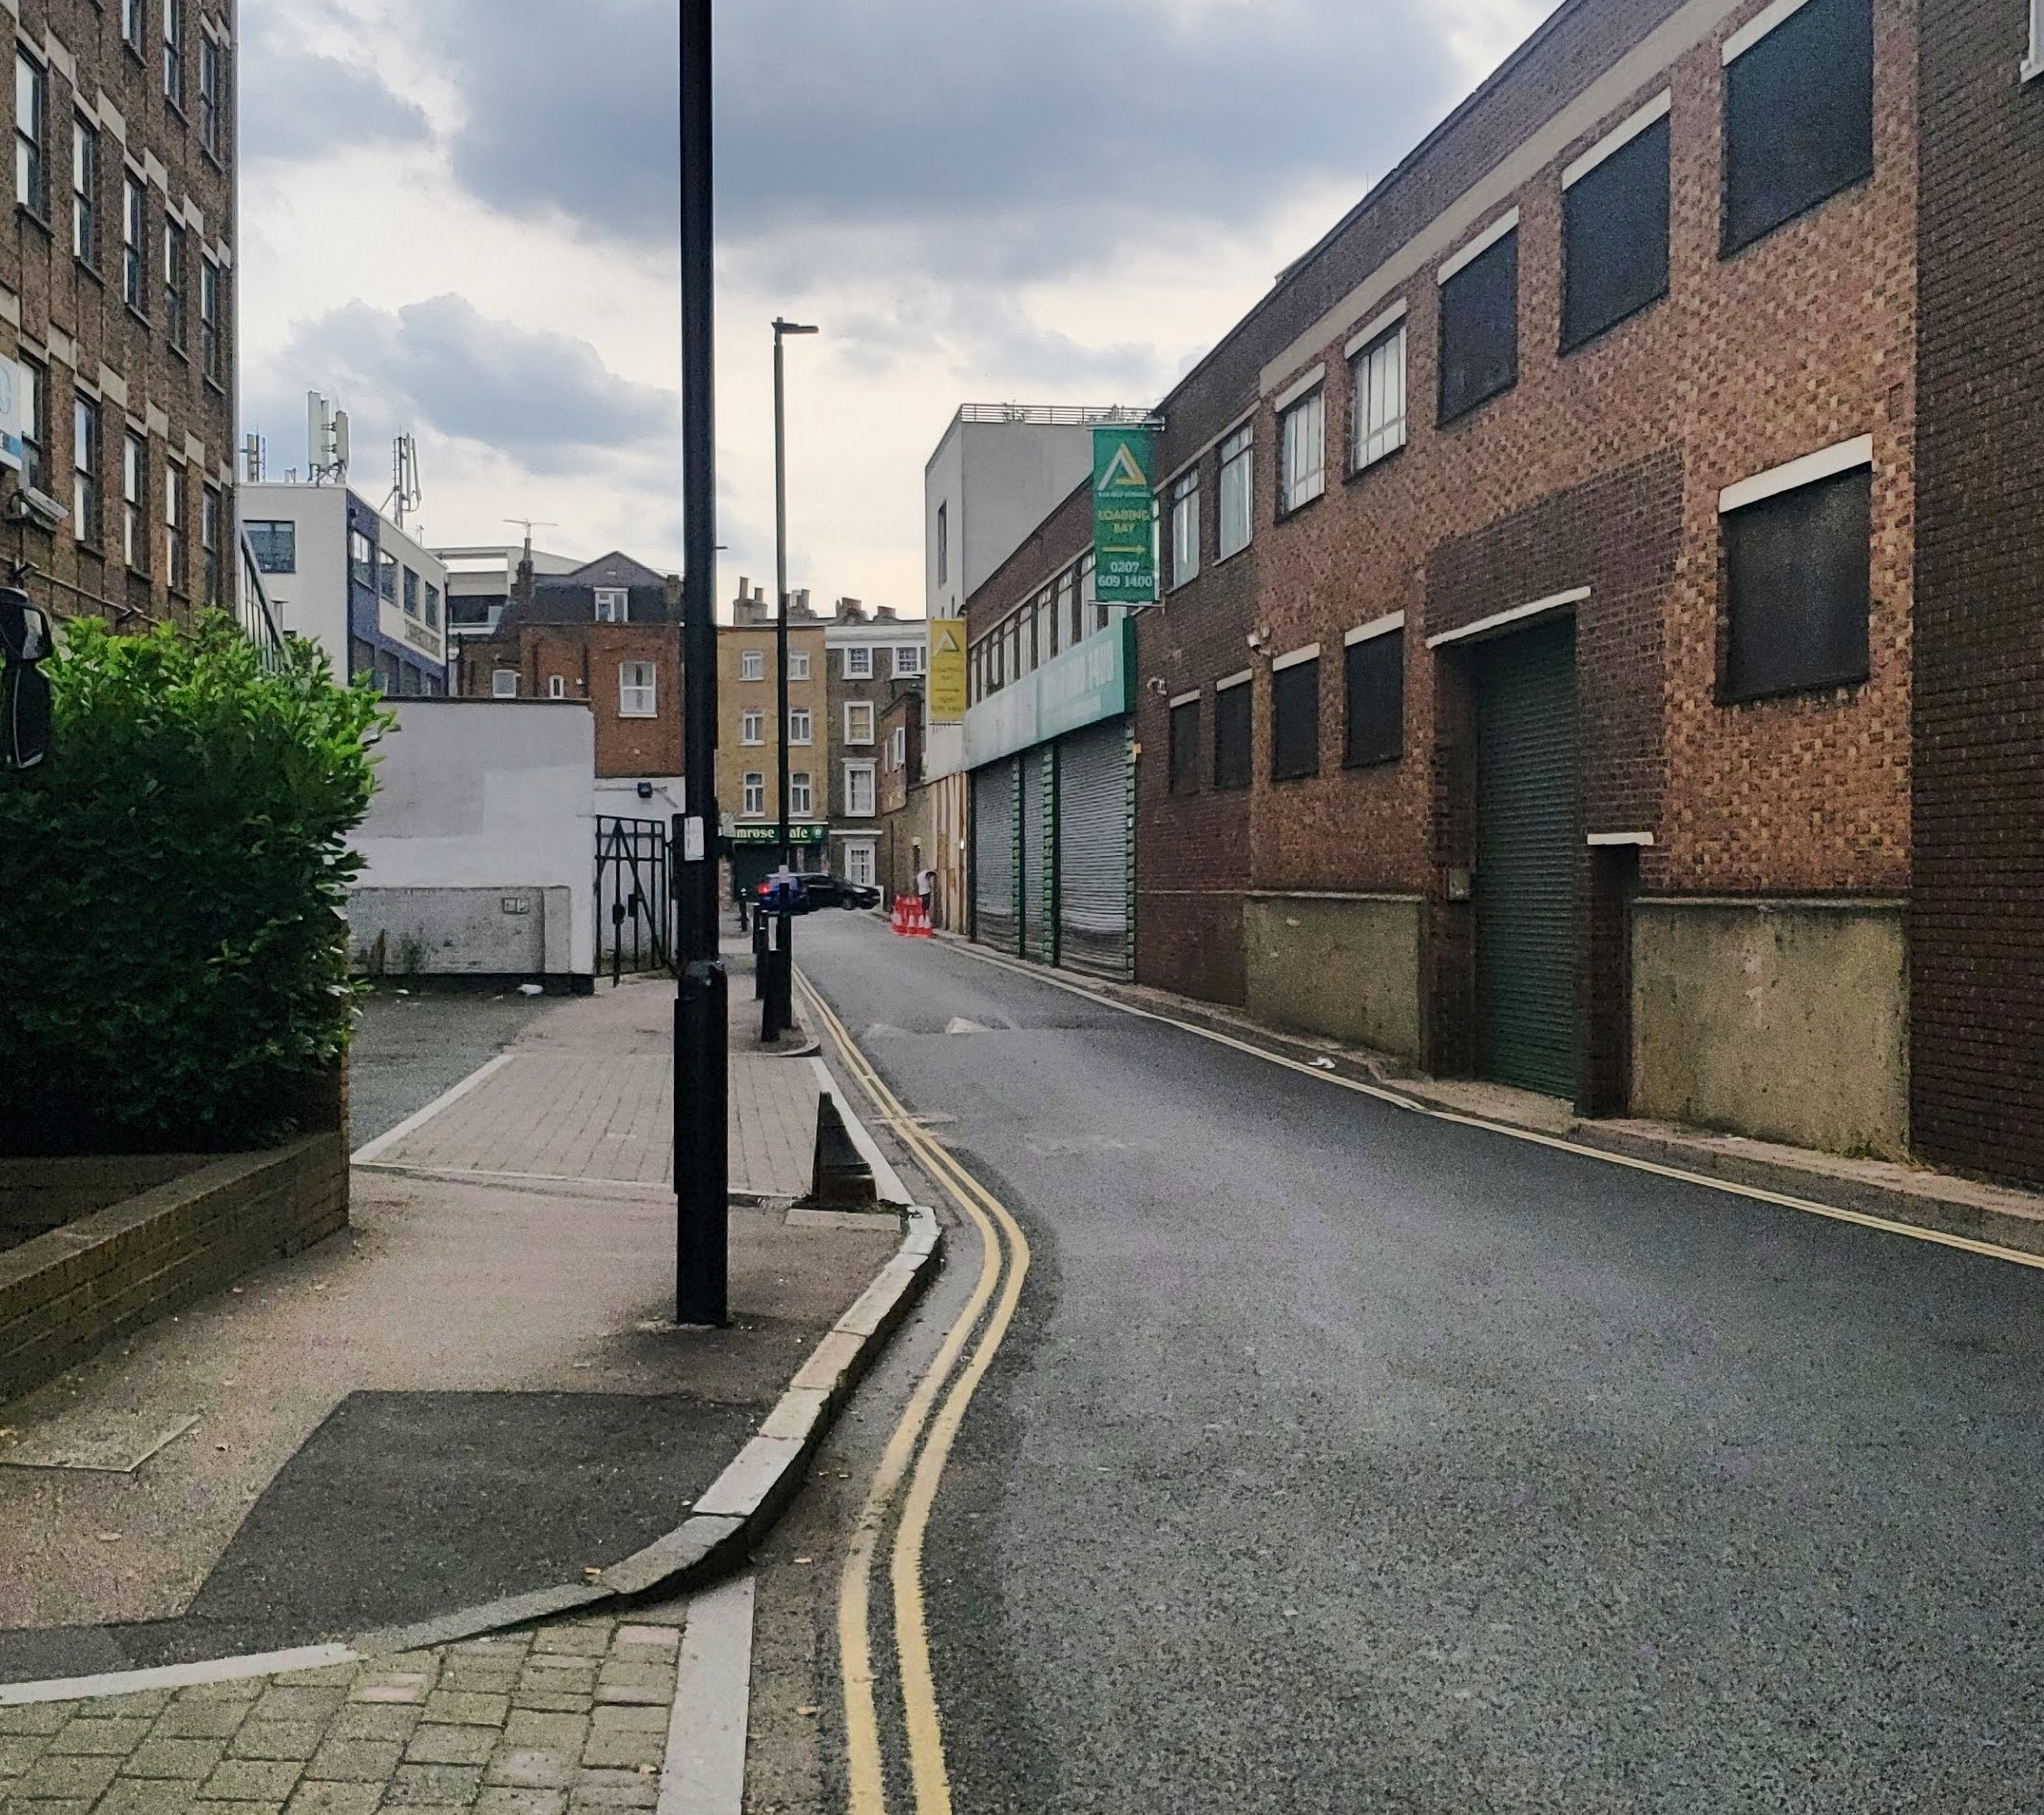
\includegraphics[width=0.6\textwidth]{brandon_rd_cropped}
\caption{image of quietway}
\end{figure}

\begin{figure}
\centering
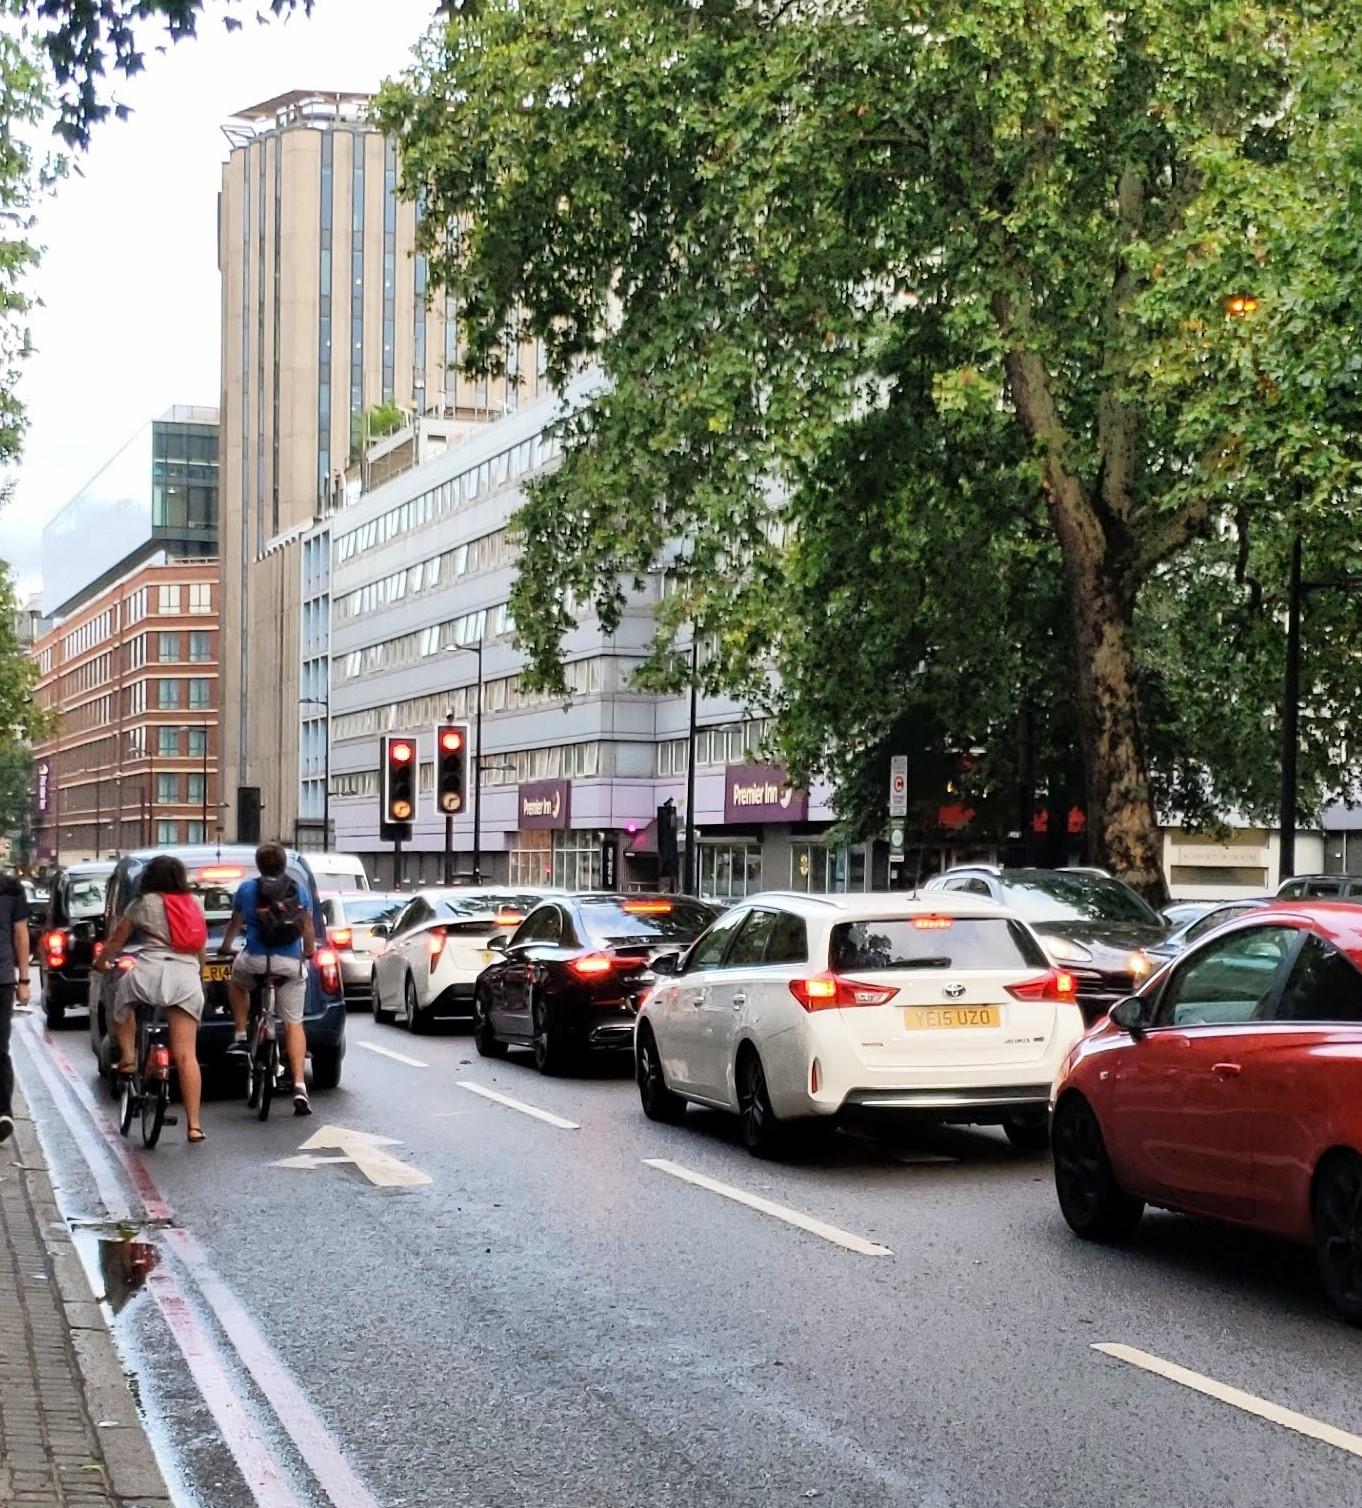
\includegraphics[width=0.6\textwidth]{euston_rd_cropped}
\caption{An image of Euston Road}
\label{fig:euston}
\end{figure}

\subsection{Transport for London Cycling Infrastructure Database}

\cite{tflcid}

This data was in the process of being publishing during the period of research for this work. 

description

possible uses

addition to OSM

osm effort to integrate
%https://wiki.openstreetmap.org/wiki/TfL_Cycling_Infrastructure_Database

\subsection{QUANT}

The QUANT dataset of public transport travel times was .

CITE

The of XXXX million pairs, XXXXX had not public transport link. To clean this data, the set is cut down to match the scope of the the investigation. Where there is no link between an origin destination pair, a link is constructed by combining the walking time from the origin to the node of highest degree in another LSOA where public transport is available to the destination LSOA. 

The walking speed used will be taken from google and the distance is the straightline distance between two points. This is less accurate than actually finding the walking route between the two points but this level of detail was not computationally feasible. 

\subsection{2011 Census Journey to work data}

The 2011 census asked each household where they lived, where they worked and how they traveled to work the preceding week. Thus data for origin and destination by mode of transport was available. This data will be used to help define the optimal scope. 

\cite{jtw}

The 2011 census asked questions about where people work and how they get there. 

This data is shared through the Nomis Labor Force website as multi-sheet excel pivot tables. Making the data usable required, stripping the meta data headings from each sheet, importing the book to pandas dataframe by sheet, melting from a picot table to long data with origin, destination, and count columns, adding the sheet name that identified the mode of travel as a column, appending each individual sheet together into a single dataframe, and pushing the dataframe to the sql database. 


Exact specifications for pulling data out of Nomis service

\subsection{LSOA boundaries and data}
	
where LSOA's were comprised of multiple polygons, the centroid of the largest polygon was used. 

lsoa population from mid 2011 

https://www.ons.gov.uk/peoplepopulationandcommunity/populationandmigration/populationestimates/datasets/lowersuperoutputareamidyearpopulationestimates

LSOA boundaries are available from the London Data store



https://data.london.gov.uk/dataset/statistical-gis-boundary-files-london

On maps created using these boundaries the copyright must be stated. This is
%"Contains National Statistics data © Crown copyright and database right [2015]" and "Contains Ordnance Survey data © Crown copyright and database right [2015]"
	
	
	
test citation for \cite{lsoageoms}. Did it work?
	
\subsection{Road KSI data}
	
https://www.gov.uk/government/collections/road-accidents-and-safety-statistics

https://data.london.gov.uk/dataset/pedal-cyclist-casualties-killed-and-seriously-injured

https://data.london.gov.uk/dataset/road-casualties-severity-borough


Factors preventing a closer understanding of road stress/danger. 
	Lack of traffic flow data
	lack of road network quality over time
	difficulty of defining actor behavior around time of crash
	difficulty of associating incident with edge.

works but the cictation isn't formatted correctly
\cite{cyclistksi}
	
\subsection{Data import, storage, cleaning, and joining}

data import was done in python using the csv, pandas, geopandas, json, and osmnx packages. Once the data was cleaned, it was passed to a postgres database with the postgis extension using the sqlalchemy package. Postgis was used for calculating distances, associating nodes with centroids

remove multipolygon lsoa interior rings in favor of polygon lsoa shapes

cite postgres
cite postgis
cited beaver
cite python
cite pandas
cite json
cite sqlachemy

text